% Provenance (never printed): see sources/outline_sources.md (Year 3:
% concordia and discordia; 40Ar/39Ar step heating; Sm-Nd model ages;
% cosmogenic nuclides; fission tracks and (U-Th)/He). Brief:
% sources/book5/BRIEFS.md, ch. 13. Curves from figdata/bachelor-3/
% concordia.py, arar_spectrum.py, model_ages.py, cosmogenic.py. Exercise and
% problem values in the Book 5 scratch calculator calc/ch13.py. The zircons,
% the biotite spectrum, the Nd sample and the helium ages of the Varden
% granite are invented, consistent with the Year 1 volume's granite of 310 Ma.
\chapter{التأريخ المتقدّم}\label{ch:b3:advanced-geochronology}

بلورة من الزركون طولها عُشر ملليمتر أبقت ساعتين تعملان منذ تبلور الغرانيت الذي تحويه:
اليورانيوم-238 المتفكّك إلى الرصاص-206، واليورانيوم-235 المتفكّك إلى الرصاص-207.
عندما تتّفق الساعتان يكون العمر بلا شكّ.
وعندما تختلفان يمكن تأريخ الاختلاف نفسه: فقد خسرت البلورة جزءًا من رصاصها في حدث لاحق،
وإذا قُرئت الساعتان معًا أعطتا عمر الغرانيت وعمر ذلك الحدث.
يقرأ هذا الفصل ساعات عدّة في وقت واحد: في اليورانيوم والرصاص، وفي الأرغون، وفي النيوديميوم،
وفي آثار الانشطار والهليوم،
وفي الذرّات النادرة التي تصنعها الأشعة الكونية،
ويبيّن إلى أيّ مدى يمكن الوثوق بكلّ عمر.

\begin{recall}
التفكّك الإشعاعي، ومعادلة العمر، والإيزوكرون ونسبته الابتدائية،
وخطّ المربعات الصغرى، والتفكّك المتفرّع، وعمر البوتاسيوم-الأرغون،
ودرجة حرارة الإغلاق وعمر التبرّد، ترد في مجلد السنة الأولى، في فصله عن
التأريخ الإشعاعي؛ أمّا صيغة التعرية المستقرّة للنويدات الكونية المنشأ فترد
في فصله عن التعرية والنقل. ويرد الخزّان الكوندريتي المنتظم،
وترميز إبسيلون والوشاح المستنفد في مجلد السنة الثانية، في فصله
عن الجيوكيمياء النظيرية؛ أمّا التأيّن الحراري وقياس الطيف الكتلي متعدّد المجمّعات
فيردان في فصله عن طرائق الحقل والمختبر. ويرد التأريخ الحراري
والعلاقة بين العمر والارتفاع في \cref{ch:b3:orogenic-wedges}.
\end{recall}

\section{اليورانيوم والرصاص والكونكورديا}\label{sec:b3:advanced-geochronology:upb}

لليورانيوم نظيران طويلا العمر. يتفكّك اليورانيوم-238 عبر سلسلة من النويدات الابنة قصيرة العمر
إلى الرصاص-206 بثابت $\lambda_{238} =
\qty{1.55125e-10}{yr^{-1}}$؛ ويتفكّك اليورانيوم-235 إلى الرصاص-207 بثابت $\lambda_{235}
= \qty{9.8485e-10}{yr^{-1}}$، أي أسرع بست مرّات. ونسبتهما الحالية هي
$^{235}\mathrm{U}/^{238}\mathrm{U} = 0.0072567$، أو $^{238}\mathrm{U}/^{235}\mathrm{U}
= 137.8$، وهي النسبة نفسها في كلّ صخرة أرضية. يستوعب الزركون، $\mathrm{ZrSiO_4}$،
كمّيات كبيرة من اليورانيوم وقليلة جدًّا من الرصاص عند نموّه، ويقاوم التجوية
ويصمد أمام التحوّل، وأغلب رصاصه مُشعّ المنشأ.
% ledger: amherst:constants, tulane:upb-zircon

لنكتب $x = {}^{207}\mathrm{Pb}^*/{}^{235}\mathrm{U}$ و$y =
{}^{206}\mathrm{Pb}^*/{}^{238}\mathrm{U}$ للنسبتين الحاليتين للرصاص المُشعّ المنشأ إلى أمّه.
ويعطي كلّ منهما عمرًا، $t_{206} = \ln(1 + y)/\lambda_{238}$
و$t_{207} = \ln(1 + x)/\lambda_{235}$.

\begin{definition}[الكونكورديا، الديسكورديا، التقاطعات، مخطط تيرا--فاسربورغ]
\label{def:b3:advanced-geochronology:concordia}
\emph{الكونكورديا}\index{الكونكورديا} هي المنحنى في المستوى $(x, y)$
الذي يتساوى عنده عمرا اليورانيوم--الرصاص. و\emph{الديسكورديا}\index{الديسكورديا}
هو خطّ مستقيم تصطفّ على امتداده التحليلات المتقاطعة لمجموعة واحدة من البلورات؛
وتقاطعاته مع الكونكورديا هي
\emph{التقاطع العلوي}\index{التقاطع العلوي} (الأقدم)
و\emph{التقاطع السفلي}\index{التقاطع السفلي} (الأحدث).
أمّا \emph{مخطط تيرا--فاسربورغ}\index{مخطط تيرا--فاسربورغ} فيرسم
$X = {}^{238}\mathrm{U}/{}^{206}\mathrm{Pb}^*$ مقابل $Y =
{}^{207}\mathrm{Pb}^*/{}^{206}\mathrm{Pb}^*$.
\end{definition}

\begin{theorem}[الكونكورديا]\label{thm:b3:advanced-geochronology:concordia}
بلورة بقيت مغلقة أمام اليورانيوم والرصاص منذ تكوّنها، أي منذ زمن
$t$ مضى، تقع عند
\[
C(t) = \bigl(e^{\lambda_{235}t} - 1,\; e^{\lambda_{238}t} - 1\bigr).
\]
مع ازدياد $t$ يصعد المنحنى مقابل $x$ بصورة أبطأ فأبطأ: ميله،
$\mathrm dy/\mathrm dx = (\lambda_{238}/\lambda_{235})\,e^{(\lambda_{238} -
\lambda_{235})t}$، يتناقص من $\lambda_{238}/\lambda_{235} = 0.1575$ عند
المبدأ، لذا \omterm{def:b3:advanced-geochronology:concordia}{فالكونكورديا} مقعّرة باتجاه المحور $x$.
\end{theorem}

\begin{proof}
لكلّ أمّ، عدد الذرّات الابنة المشعّة المنشأ لكلّ ذرّة أمّ متبقّية هو
$e^{\lambda t} - 1$، وهي معادلة العمر في مجلد السنة الأولى. وبتفاضل
الإحداثيين كليهما بالنسبة إلى $t$ والقسمة نحصل على الميل؛ وبما أنّ
$\lambda_{235} > \lambda_{238}$، فإنّ الميل يتناقص مع $t$.
\end{proof}

الرصاص أيون كبير لا يستقرّ جيّدًا في شبكة الزركون. وفي الأجزاء من
البلورة المتضرّرة بإشعاعها الذاتي، يمكن أن يخرج أثناء حدث لاحق من
التسخين أو دوران السوائل.
% ledger: tulane:upb-zircon

\begin{theorem}[فقد الرصاص المتقطّع يعطي وترًا]\label{thm:b3:advanced-geochronology:discordia}
بلورة تكوّنت قبل زمن $t_1$، وفقدت قبل زمن $t_2$ كسرًا $f$
من رصاصها المشعّ المنشأ، وبقيت مغلقة فيما عدا ذلك، وتقع اليوم عند
\[
(1 - f)\,C(t_1) + f\,C(t_2),
\]
على الوتر الواصل بين النقطتين $t_1$ و$t_2$ من \omterm{def:b3:advanced-geochronology:concordia}{الكونكورديا}. والبلورات التي
فقدت كسورًا مختلفة تقع على ذلك الوتر، وهو ديسكورديا تقاطعه العلوي
هو $t_1$ وتقاطعه السفلي هو $t_2$.
\end{theorem}

\begin{proof}
نأخذ نظام تفكّك واحدًا ثابته $\lambda$، ونعدّ لكلّ ذرّة أمّ
موجودة اليوم. قبل زمن $t_2$ كان هناك $e^{\lambda t_2}$ من ذرّات الأمّ، وكانت
الذرّات الابنة المشعّة المنشأ $e^{\lambda t_2}(e^{\lambda(t_1 - t_2)} - 1) =
e^{\lambda t_1} - e^{\lambda t_2}$. أمّا الحدث فقد ترك $(1 - f)(e^{\lambda t_1} -
e^{\lambda t_2})$؛ ومنذ ذلك الحين أنتجت الأمّ $e^{\lambda t_2} - 1$ إضافية.
والمجموع هو $(1 - f)(e^{\lambda t_1} - 1) + f(e^{\lambda t_2} - 1)$. ويسلك نظيرا الرصاص
سلوكًا كيميائيًّا متشابهًا، فإنّ $f$ واحدة لكليهما،
ويجتمع الإحداثيان في النقطة المذكورة.
\end{proof}

\begin{omfigure}
\begin{tikzpicture}
\begin{groupplot}[group style={group size=2 by 1, horizontal sep=1.7cm},
  omrecord, width=0.47\linewidth, height=0.42\linewidth, title style={font=\small},
  tick label style={font=\scriptsize}, label style={font=\small}]
\nextgroupplot[title={(أ) مخطط الكونكورديا},
  xlabel={$^{207}\mathrm{Pb}^*/^{235}\mathrm{U}$}, ylabel={$^{206}\mathrm{Pb}^*/^{238}\mathrm{U}$},
  xmin=0.04, xmax=0.44, ymin=0.006, ymax=0.06,
  xtick={0.1,0.2,0.3,0.4}, xticklabels={0.1,0.2,0.3,0.4},
  ytick={0.01,0.02,0.03,0.04,0.05}, yticklabels={0.01,0.02,0.03,0.04,0.05},
  scaled ticks=false]
% computed in figdata/bachelor-3/concordia.py
\addplot[black, thick] table[x=xw, y=yw] {figdata/out/bachelor-3-concordia-curve.dat};
\addplot[black, only marks, mark=*, mark size=1.4pt, nodes near coords={\scriptsize\pgfmathprintnumber[fixed, precision=0]{\pgfplotspointmeta}},
  point meta=explicit, nodes near coords align={anchor=south east},
  restrict expr to domain={\thisrow{t}}{100:350}]
  table[x=xw, y=yw, meta=t] {figdata/out/bachelor-3-concordia-ticks.dat};
\addplot[omDef, thick, densely dashed] table[x=x, y=y] {figdata/out/bachelor-3-concordia-line.dat};
\addplot[red!70!black, only marks, mark=diamond*, mark size=2pt] table[x=x, y=y] {figdata/out/bachelor-3-concordia-zircons.dat};
\nextgroupplot[title={(ب) مخطط تيرا--فاسربورغ},
  xlabel={$^{238}\mathrm{U}/^{206}\mathrm{Pb}^*$}, ylabel={$^{207}\mathrm{Pb}^*/^{206}\mathrm{Pb}^*$},
  xmin=15, xmax=75, ymin=0.0465, ymax=0.0535,
  ytick={0.047,0.049,0.051,0.053}, yticklabels={0.047,0.049,0.051,0.053},
  scaled ticks=false]
\addplot[black, thick] table[x=xtw, y=ytw] {figdata/out/bachelor-3-concordia-curve.dat};
\addplot[black, only marks, mark=*, mark size=1.4pt, nodes near coords={\scriptsize\pgfmathprintnumber[fixed, precision=0]{\pgfplotspointmeta}},
  point meta=explicit, nodes near coords align={anchor=north east},
  restrict expr to domain={\thisrow{t}}{100:250}]
  table[x=xtw, y=ytw, meta=t] {figdata/out/bachelor-3-concordia-ticks.dat};
\addplot[omDef, thick, densely dashed] table[x=xtw, y=ytw] {figdata/out/bachelor-3-concordia-twline.dat};
\addplot[red!70!black, only marks, mark=diamond*, mark size=2pt] table[x=xtw, y=ytw] {figdata/out/bachelor-3-concordia-zircons.dat};
\end{groupplot}
\end{tikzpicture}

\par\smallskip{\small (أ) \omterm{def:b3:advanced-geochronology:concordia}{الكونكورديا}، مع أعمارها بالملايين من السنين،
خمسة زركونات مصطنعة غير متوافقة من جرانيت واحد (باللون الأحمر؛ قطوع الخطأ الناقصة لها
أصغر من الرموز)، مصطفّةً على خطّ \omterm{def:b3:advanced-geochronology:concordia}{الديسكورديا} (المتقطّع) الذي
يلتقي \omterm{def:b3:advanced-geochronology:concordia}{بالكونكورديا} قرب 311 و\qty{100}{\Ma}. (ب) الزركونات نفسها والخط نفسه
في \omterm{def:b3:advanced-geochronology:concordia}{مخطط تيرا--فاسربورغ}، حيث يبقى \omterm{def:b3:advanced-geochronology:concordia}{الديسكورديا} خطًّا
مستقيمًا.}\label{fig:b3:advanced-geochronology:concordia}
\end{omfigure}
% ledger: amherst:constants

تُحسب التقاطعات حيث $a + b\,x(t) = y(t)$، وهي معادلة في $t$ تُحلّ
بطريقة نيوتن: مع $g(t) = e^{\lambda_{238}t} - 1 - a -
b(e^{\lambda_{235}t} - 1)$ و$g'(t) = \lambda_{238}e^{\lambda_{238}t} -
b\lambda_{235}e^{\lambda_{235}t}$، نكرّر $t \leftarrow t - g/g'$ انطلاقًا من تخمين
قرب كلّ تقاطع. تهمّ ثلاث خصائص للنتيجة في التطبيق.
أوّلًا، لا يكون \omterm{def:b3:advanced-geochronology:concordia}{التقاطع العلوي} دقيقًا إلّا إذا قطع \omterm{def:b3:advanced-geochronology:concordia}{الديسكورديا}
\omterm{def:b3:advanced-geochronology:concordia}{الكونكورديا} بزاوية كبيرة. \omterm{def:b3:advanced-geochronology:concordia}{الديسكورديا} الفتيّ، كما في الشكل أعلاه، يمتدّ
تقريبًا على طول \omterm{def:b3:advanced-geochronology:concordia}{الكونكورديا}، ويكفي تغيّرٌ صغير في ميله لنقل التقاطع
بعيدًا. ثانيًا، إذا كان فقد الرصاص حديثًا، $t_2 = 0$، يمرّ \omterm{def:b3:advanced-geochronology:concordia}{الديسكورديا}
بنقطة الأصل، ويكون لكلّ بلّورة النسبة نفسها
$^{207}\mathrm{Pb}^*/^{206}\mathrm{Pb}^*$،
\[
\frac{^{207}\mathrm{Pb}^*}{^{206}\mathrm{Pb}^*} = \frac{1}{137.8}\,
\frac{e^{\lambda_{235}t_1} - 1}{e^{\lambda_{238}t_1} - 1},
\]
وهي تعطي $t_1$ دون الحاجة إلى اليورانيوم، وهو عمر الرصاص--الرصاص. ثالثًا، يتحوّل الخطّ في مخطّط \omterm{def:b3:advanced-geochronology:concordia}{الكونكورديا}،
$x = (y - a)/b$، في إحداثيات تيرا--فاسربورغ
$Y = (1 - aX)/(137.8\,b)$، إلى خطّ مجدّدًا. يستخدم مخطّط تيرا--فاسربورغ نسبًا
قيست مباشرةً دون الحاجة إلى حساب اليورانيوم-235 من اليورانيوم-238، ويقع مزيجٌ
مع الرصاص الشائع، غير المشعّ وغنيّ بالرصاص-207، على خطّ
يبلغ محور $Y$ عند نسبة
الرصاص الشائع.

تُقاس أعمار اليورانيوم--الرصاص بطريقتين. البلّورات المفردة أو الشظايا،
تُذاب بعد إزالة المناطق المتضرّرة بالإذابة الجزئية،
وفصل الرصاص واليورانيوم منها، تُقاس بمطياف الكتلة بالتأيّن الحراري،
وهي أدقّ أعمار في الجيولوجيا. تُقاس البقع بعرض بضعة عشرات
من الميكرومترات في موضعها، بمسبار أيوني أو بالاستئصال بالليزر،
أقلّ دقّةً، لكنّها تُقاس منطقةً تلو أخرى عبر بلّورة نمت خلال
عدّة أحداث.

\begin{inthelab}[مختبر التأريخ الجيولوجي]
\begin{minipage}[t]{0.55\linewidth}\vspace{0pt}
يبدأ تأريخ الزركون بصخرة مسحوقة وينتهي في مختبر نظيف. يفصل الباحثون
الزركونات حسب الكثافة والمغناطيسية، ويختارون أوضح البلّورات
تحت المجهر الثنائي العينيّة، ويصوّرون تدرّجها.
تُذاب البلّورات جزئيًّا لإزالة مناطقها المتضرّرة، ثم تُذاب
كلّيًّا بمُنشِّط من نظائر معلومة، ويُفصل اليورانيوم والرصاص
على أعمدة راتنجية دقيقة، في هواء مُرشَّح لاستبعاد
غبار الرصاص. يقيس مطياف الكتلة نِسَب النظائر. وتسلك عيّنات الأرغون
مسارًا مختلفًا: مفاعلًا، ثم خطَّ غازات يُسخَّن فيه كلّ طور بالليزر،
ويُنقّى الأرغون قبل مطياف الكتلة.
\end{minipage}\hfill
\begin{minipage}[t]{0.42\linewidth}\vspace{0pt}
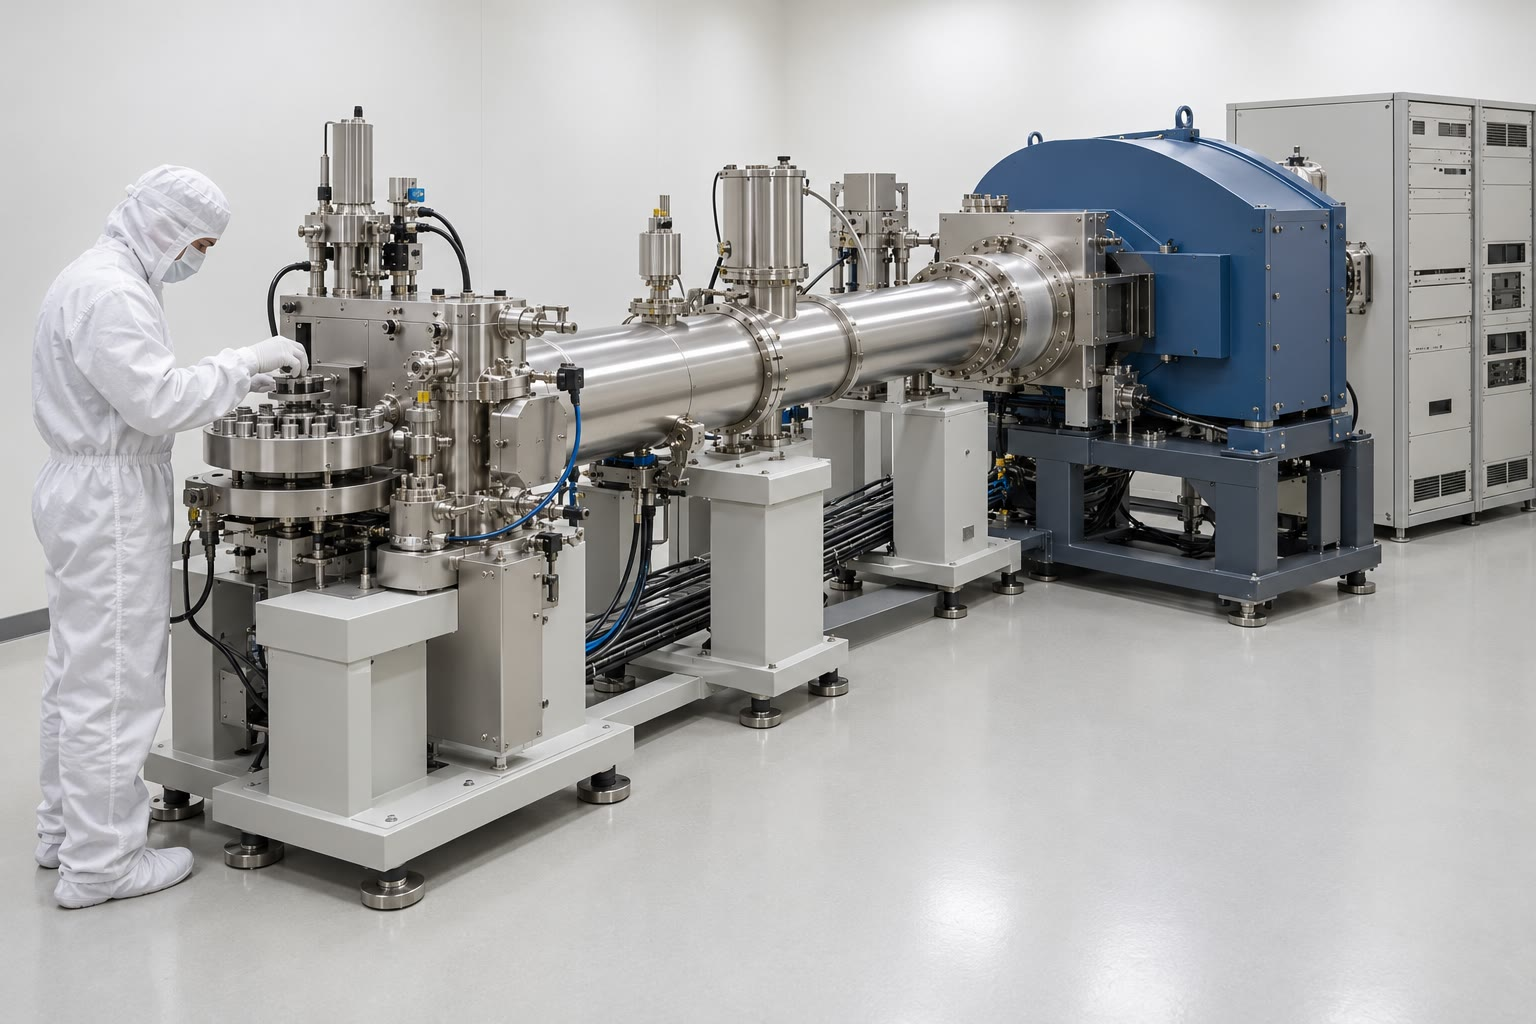
\includegraphics[width=\linewidth]{images/book5/ai/b3-mass-spec-lab.jpg}

{\scriptsize مطياف الكتلة في مختبر نظيف: برج العيّنات إلى اليسار،
وأنبوب الطيران والمغناطيس الكهربائي (رسم توضيحي مولَّد بالذكاء
الاصطناعي).}
\end{minipage}
\end{inthelab}

\section{التأريخ بطريقة الأرغون--الأرغون}\label{sec:b3:advanced-geochronology:arar}

تقيس طريقة البوتاسيوم--الأرغون الواردة في مجلد السنة الأولى البوتاسيوم والأرغون
في عيّنتين جزئيّتين منفصلتين من معدن. وتقيس طريقة الأرغون--الأرغون الأرغونَ وحده،
في عيّنة جزئية واحدة، على هيئة نِسب نظائر. وتُشعَّع العيّنة
بنيوترونات سريعة في قلب مفاعل نووي، حيث يحوّل التفاعل
$^{39}\mathrm{K}(n,p)^{39}\mathrm{Ar}$ نسبةً ثابتةً من البوتاسيوم-39 إلى
الأرغون-39، وهو بديلٌ عن البوتاسيوم. ويُشعَّع بجوارها معدن معلوم العمر،
وهو المراقِب.
% ledger: nmgrl:arar, amherst:arar

\begin{definition}[التأريخ بطريقة الأرغون--الأرغون، العامل J، طيف الأعمار، عمر الهضبة]
\label{def:b3:advanced-geochronology:arar}
\emph{التأريخ بطريقة $^{40}\mathrm{Ar}/^{39}\mathrm{Ar}$}\index{التأريخ بطريقة $^{40}\mathrm{Ar}/^{39}\mathrm{Ar}$}
يؤرّخ معدنًا يحوي البوتاسيوم بالنسبة $R =
{}^{40}\mathrm{Ar}^*/{}^{39}\mathrm{Ar}_{\mathrm K}$ للأرغون-40 المشعّ إلى
الأرغون-39 المتكوّن من بوتاسيومه بالتشعيع النيوتروني.
\emph{العامل J}\index{العامل J} للتشعيع هو $J = (e^{\lambda
t_m} - 1)/R_m$، ويُحسب انطلاقًا من مراقِب معلوم العمر $t_m$ والنسبة المقيسة
$R_m$، حيث $\lambda$ ثابت الاضمحلال الكلّي للبوتاسيوم-40. وحين تُزال غازات العيّنة
على خطوات متزايدة الحرارة، يرسم \emph{طيف
الأعمار}\index{طيف الأعمار} عمرَ كلّ خطوة مقابل
الكسر التراكمي للأرغون-39 المحرَّر. أمّا \emph{عمر
الهضبة}\index{عمر الهضبة} فهو المتوسّط المرجّح لأعمار خطوات متتالية
تتّفق ضمن حدود عدم اليقين فيها، وتحرّر جزءًا كبيرًا من الأرغون-39.
\end{definition}

\begin{theorem}[عمر الأرغون--الأرغون]\label{thm:b3:advanced-geochronology:arar}
يكون لعيّنةٍ مُشعَّعةٍ مع مراقِب العمرُ
\[
t = \frac1\lambda\ln(1 + JR).
\]
\end{theorem}

\begin{proof}
الأرغون المشعّ هو $^{40}\mathrm{Ar}^* = (\lambda_e/\lambda)\,
{}^{40}\mathrm{K}\,(e^{\lambda t} - 1)$، بحسب الاضمحلال المتفرّع الوارد في
مجلد السنة الأولى. والأرغون-39 المتكوّن هو $^{39}\mathrm{Ar}_{\mathrm K} =
{}^{39}\mathrm{K}\,\Phi$، حيث يجمع $\Phi$ الجرعة النيوترونية
والمقطع العرضي للتفاعل. إذن $R = (e^{\lambda t} - 1)/J$ مع $J =
\lambda\,\Phi\,{}^{39}\mathrm{K}/(\lambda_e\,{}^{40}\mathrm{K})$. تكون النسبة
$^{40}\mathrm{K}/^{39}\mathrm{K}$ هي نفسها في كلّ البوتاسيوم، و$\Phi$ نفسه
لعيّنتين شُعّعتا جنبًا إلى جنب، فيكون $J$ واحدًا للعيّنة
والمراقِب؛ ويُعطى بعمر المراقِب ونسبته، وبعكس $R$ نحصل على
$t$.
\end{proof}

الثوابت هي ثوابت طريقة البوتاسيوم--الأرغون، $\lambda =
\qty{5.543e-10}{yr^{-1}}$. ويُستعمل مراقِب شائع، هو السانيدين من تُفّ بركاني
مؤرَّخٌ عند \qty{28.201}{\Ma}؛ ونسبة المراقِب $R_m = 1.3129$ تعطي $J =
0.01200$. يُطرح الأرغون الجوّي، ذو النسبة $^{40}\mathrm{Ar}/^{36}\mathrm{Ar} = 295.5$،
مستعملًا الأرغون-36 المقيس في كلّ خطوة، ويُصحَّح الأرغون المتكوّن بالنيوترونات
من الكالسيوم ومن البوتاسيوم نفسه بأملاح شُعّعت
في الحزمة نفسها.
% ledger: schaen20:monitors, amherst:constants, nmgrl:arar

التسخين المتدرّج هو نقطة قوّة الطريقة. تُسخَّن العيّنة في فرن
أو بالليزر على خطوات متزايدة الحرارة، وتعطي كلّ خطوة عمرًا.
إن بقي المعدن مغلقًا منذ تبرّده، تتّفق الخطوات كلّها: يكون الطيف
مسطّحًا. وإن فقد الأرغون من أطراف حبيباته، فإنّ الخطوات الأولى، التي
تأتي من الأطراف، تكون أحدث، وترتفع الأعمار كدرج نحو
هضبة تعطيها لُبوب الحبيبات. ومن معايير الهضبة الموصى بها أن تكون
خمس خطوات متتالية على الأقل تحمل أكثر من \qty{50}{\percent} من
الأرغون-39، دون أيّ اتجاه بينها؛ وتُفسَّر خطوات الدرج ذات الحرارة المنخفضة
عادةً بوصفها فقدانًا للأرغون المشعّ المنشأ. أمّا الأرغون الزائد، المحبوس من
مائع عند نمو المعدن، فيفعل العكس: يجعل بعض الخطوات أقدم من اللازم،
وغالبًا الأولى والأخيرة، في طيف على شكل سرج. ومجموع الخطوات كلّها،
أي عمر الغاز الكلّي، هو ما كان سيعطيه عمر البوتاسيوم--الأرغون: متوسّطًا
يُخفي التاريخ.
% ledger: schaen20:plateau, nmgrl:arar

\begin{omfigure}
\begin{tikzpicture}
\begin{groupplot}[group style={group size=2 by 1, horizontal sep=1.5cm},
  omrecord, height=0.38\linewidth, title style={font=\small},
  xlabel={الأرغون $^{39}\mathrm{Ar}$ المتحرّر تراكميًّا \babelsublr{(\unit{\percent})}},
  tick label style={font=\scriptsize}, label style={font=\small}]
\nextgroupplot[title={(أ) الطيف كاملًا}, width=0.52\linewidth,
  ylabel={العمر الظاهري \babelsublr{(\unit{\Ma})}}, xmin=0, xmax=100, ymin=130, ymax=320,
  xtick={0,20,40,60,80,100}, ytick={150,200,250,300}]
% computed in figdata/bachelor-3/arar_spectrum.py
\addplot[omDef, thick] table[x=cum, y=age] {figdata/out/bachelor-3-arar_spectrum-boxes.dat};
\node[font=\scriptsize, anchor=west] at (axis cs:12,180) {فقدان الأرغون};
\node[font=\scriptsize, anchor=north, red!70!black] at (axis cs:59,290) {هضبة};
\nextgroupplot[title={(ب) الهضبة مكبّرة}, width=0.44\linewidth,
  xmin=15, xmax=100, ymin=290, ymax=300, xtick={20,40,60,80,100},
  ytick={290,292,294,296,298,300}]
\addplot[name path=hi, draw=none, forget plot] table[x=cum, y=hi] {figdata/out/bachelor-3-arar_spectrum-boxes.dat};
\addplot[name path=lo, draw=none, forget plot] table[x=cum, y=lo] {figdata/out/bachelor-3-arar_spectrum-boxes.dat};
\addplot[omDef!25, forget plot] fill between[of=hi and lo];
\addplot[omDef, thick] table[x=cum, y=age] {figdata/out/bachelor-3-arar_spectrum-boxes.dat};
\draw[red!70!black, thick] (axis cs:18,296.1) -- (axis cs:100,296.1);
\node[font=\scriptsize, anchor=south, red!70!black] at (axis cs:59,290.3) {\foreignlanguage{arabic}{هضبة \mbox{\textdir TLT \qty[separate-uncertainty=true]{296.1 \pm 0.8}{\Ma}}}};
\end{groupplot}
\end{tikzpicture}

\par\smallskip{\small \omterm{def:b3:advanced-geochronology:arar}{طيف الأعمار} المُفترَض لمعدن البيوتيت من الغرانيت في
الشكل الأول: تُرسم كلّ خطوة عند عمرها، ويمثّل عرضها حصّتها من
الأرغون-39 المتحرّر منها. (أ) ترتفع ثلاث خطوات ذات حرارة منخفضة كدرج نحو
هضبة. (ب) الخطوات السبع للهضبة، التي تحوي \qty{82}{\percent} من
الأرغون-39، مع مداها عند انحرافين معياريين (مظلَّلة)، \omterm{def:b3:advanced-geochronology:arar}{وعمر الهضبة}
(بالأحمر).}\label{fig:b3:advanced-geochronology:spectrum}
\end{omfigure}

\section{أعمار النموذج للنيوديميوم}\label{sec:b3:advanced-geochronology:model-age}

عندما يُستخلَص مصهور من الوشاح لتكوين القشرة القارّية، يبقى السماريوم،
الأكثر توافقًا، في المصدر أكثر من النيوديميوم: تملك القشرة الجديدة نسبة أدنى
$^{147}\mathrm{Sm}/^{144}\mathrm{Nd}$ من مصدرها، نحو 0.13 لمعظم
الصخور القشرية، مقابل 0.1966 للخزّان الكوندريتي. ونسبة
$^{143}\mathrm{Nd}/^{144}\mathrm{Nd}$ فيها تنمو ببطء أكبر. وما إن تتكوّن صخرة قشرية، تميل
إلى الحفاظ على نسبة السماريوم--النيوديميوم، عبر التعرية،
والترسيب بل وحتى إعادة الانصهار، فيحفظ نيوديميومها ذكرى وقت مغادرته
الوشاح.
% ledger: white08:model-age, white:chur

\begin{definition}[العمر النموذجي]\label{def:b3:advanced-geochronology:model-age}
\emph{العمر النموذجي}\index{العمر النموذجي} لصخرة في نظام نظيري هو الزمن
الذي تساوي فيه نسبتها، مُسقَطةً إلى الخلف بنسبة الأمّ--البنت الحالية،
نسبة خزّان نموذجي. وفي حالة النيوديميوم، يعتمد $T_{\mathrm{CHUR}}$
على الخزّان الكوندريتي المتجانس، و$T_{\mathrm{DM}}$ على الوشاح
المستنفد.
\end{definition}

\begin{theorem}[العمر النموذجي]\label{thm:b3:advanced-geochronology:model-age}
لعيّنة ذات النسب الحالية $I_s = {}^{143}\mathrm{Nd}/^{144}\mathrm{Nd}$
و$R_s = {}^{147}\mathrm{Sm}/^{144}\mathrm{Nd}$، تُقارَن بخزّان ذي النسب الحالية
$I_m$ و$R_m$، يكون لها \omterm{def:b3:advanced-geochronology:model-age}{العمر النموذجي}
\[
T = \frac1\lambda\ln\left(1 + \frac{I_s - I_m}{R_s - R_m}\right),
\qquad \lambda = \lambda_{147}.
\]
\end{theorem}

\begin{proof}
كان لنظام مغلق قبل الزمن $T$ النسبة $I - R(e^{\lambda T} - 1)$: معادلة
الإيزوكرون مقروءةً بالعكس. وبمساواة هذا للعيّنة
والخزّان نجد $I_s - I_m = (R_s - R_m)(e^{\lambda T} - 1)$.
\end{proof}

مع $\lambda_{147} = \qty{6.524e-12}{yr^{-1}}$، الخزّانان هما
الكوندريتي بقيمة 0.512638 و0.1966 اليوم، والوشاح المستنفد،
بقيمة 0.51315 اليوم، أي نحو $\varepsilon_{\mathrm{Nd}} = +10$، وهي القيمة التي يعطيها تطوّر مغلق
من القيم الكوندريتية منذ \qty{4.55}{\Ga} النسبة
$^{147}\mathrm{Sm}/^{144}\mathrm{Nd} = 0.2137$. وغرانيت مُفترَض ذو
$I_s = 0.511900$ و$R_s = 0.1100$ يملك $\varepsilon_{\mathrm{Nd}} = -14.4$
اليوم، و$T_{\mathrm{CHUR}} = \qty{1.30}{\Ga}$ و$T_{\mathrm{DM}} =
\qty{1.84}{\Ga}$. ويقرأ الشكل أدناه القيمتين. ويُعدّ عمر الوشاح المستنفد
التقديرَ الأفضل، لأنّ القشرة تُستخلَص من وشاح مستنفد أصلًا؛
 فهو متوسّط العمر الذي غادر فيه نيوديميوم العيّنة الوشاح،
وهو عمر إقامتها القشرية. ويحدّ منه قيدان: يجب ألّا تكون القشرة قد غيّرت
نسبة السماريوم--النيوديميوم منذ ذلك، وأنّ الصخرة المكوّنة بخلط
قشرة قديمة بمصهورات وشاح جديد لها عمر نموذجي وسيط لا معنى له.
% ledger: villa20:sm147, white:chur, white08:model-age

\begin{omfigure}
\begin{tikzpicture}
\begin{axis}[omrecord, width=0.72\linewidth, height=0.38\linewidth,
  xlabel={الزمن قبل الحاضر \babelsublr{(\unit{\Ga})}}, ylabel={$\varepsilon_{\mathrm{Nd}}$},
  xmin=0, xmax=2.5, ymin=-17, ymax=13, x dir=reverse,
  xtick={0,0.5,1,1.5,2,2.5}, xticklabels={0,0.5,1,1.5,2,2.5},
  tick label style={font=\scriptsize}, label style={font=\small},
  legend style={font=\scriptsize, at={(0.5,1.03)}, anchor=south, legend columns=3, legend cell align=left}]
% computed in figdata/bachelor-3/model_ages.py
\addplot[omDef, thick] table[x=t, y=eps_dm] {figdata/out/bachelor-3-model_ages-evolution.dat};
\addlegendentry{الوشاح المستنفد}
\addplot[black, thick, densely dashed] coordinates {(0,0) (2.5,0)};
\addlegendentry{CHUR}
\addplot[red!70!black, thick] table[x=t, y=eps_sample] {figdata/out/bachelor-3-model_ages-evolution.dat};
\addlegendentry{الغرانيت}
\draw[densely dotted] (axis cs:1.30,0) -- (axis cs:1.30,-17) node[above right, font=\scriptsize, rotate=90] {$T_{\mathrm{CHUR}}$};
\draw[densely dotted] (axis cs:1.84,5.4) -- (axis cs:1.84,-17) node[above right, font=\scriptsize, rotate=90] {$T_{\mathrm{DM}}$};
\end{axis}
\end{tikzpicture}

\par\smallskip{\small $\varepsilon_{\mathrm{Nd}}$ لغرانيت مفترض مُسقَط
إلى الماضي بنسبة السماريوم--النيوديميوم الخاصة به (الأحمر). يلتقي
المستودع الكوندريتي عند $T_{\mathrm{CHUR}} = \qty{1.30}{\Ga}$ والوشاح
المستنفد (الأزرق) عند $T_{\mathrm{DM}} = \qty{1.84}{\Ga}$.}\label{fig:b3:advanced-geochronology:model-age}
\end{omfigure}

\section{آثار الانشطار والهيليوم}\label{sec:b3:advanced-geochronology:low-t}

يتحلّل اليورانيوم-238 أيضًا، وذلك نادرًا جدًّا، بالانشطار التلقائي: تنشطر النواة
إلى شظيّتين تتباعدان وتتركان مسارًا من التلف في البلورة، يبلغ عرضه حتى \qty{9}{nm}
وطوله نحو \qty{23}{\micro\metre} في الأباتيت.
بعد تنميشها بالحمض تصبح المسارات مرئية تحت المجهر.
تلتئم حين تُسخَّن البلورة، عبر نحو 20 إلى \qty{350}{\celsius}،
حسب المعدن؛ وفي الأباتيت تتقلّص في نطاق التلدين الجزئي،
نحو 60 إلى \qty{120}{\celsius}، وتختفي فوق ذلك.
% ledger: kohn24:ft, sueoka19:closure

\begin{definition}[التأريخ بآثار الانشطار، تلدين الآثار]\label{def:b3:advanced-geochronology:fission-track}
\emph{التأريخ بآثار الانشطار}\index{التأريخ بآثار الانشطار} يؤرّخ معدنًا
بكثافة الآثار التي يتركها فيه الانشطار التلقائي لليورانيوم-238
مقارنةً بمحتواه من اليورانيوم. \emph{تلدين
الآثار}\index{تلدين الآثار} هو تقلّص الآثار واختفاؤها بفعل إصلاح
البلورة عند تسخينها.
\end{definition}

\begin{theorem}[عمر آثار الانشطار]\label{thm:b3:advanced-geochronology:fission-track}
ليكن $\lambda_f$ ثابت تفكّك الانشطار التلقائي، و$\lambda =
\lambda_{238}$ الثابت الكلّي، فإنّ بلورةً فيها $N_s$ من حالات الانشطار التلقائي لكلّ وحدة
حجم و$N$ ذرّة من اليورانيوم-238 لها العمر
\[
t = \frac1\lambda\ln\left(1 + \frac{\lambda}{\lambda_f}\,\frac{N_s}{N}\right).
\]
في المختبر يُقاس اليورانيوم بإحداث انشطار
اليورانيوم-235 بالنيوترونات الحرارية، ويصبح العمر
\[
t = \frac1\lambda\ln\left(1 + \lambda\,\zeta\,g\,\rho_d\,\frac{\rho_s}{\rho_i}\right),
\]
حيث $\rho_s$ و$\rho_i$ كثافتا الآثار التلقائية والمستحثّة،
و$\rho_d$ كثافة الآثار في زجاج قياس الجرعة، و$g = 0.5$ عاملًا هندسيًّا
و$\zeta$ ثابت معايرة يُحصل عليه من عيّنات معيارية معلومة العمر.
\end{theorem}

\begin{proof}
تفكّك اليورانيوم-238 $N(e^{\lambda t} - 1)$ مرّة، وكان الكسر
$\lambda_f/\lambda$ من هذه التفكّكات انشطارات: $N_s =
(\lambda_f/\lambda)N(e^{\lambda t} - 1)$، وبإعادة ترتيبها تنتج الصيغة الأولى.
تتناسب كثافتا الآثار طرديًّا مع $N_s$ ومع عدد
الانشطارات المستحثّة، $N\,\sigma\,\Phi/137.8$، حيث $\sigma$ مقطع الانشطار
لليورانيوم-235 و$\Phi$ التدفّق النيوتروني المتكامل، وهو بدوره
متناسب مع $\rho_d$. والنسبة $\rho_s/\rho_i$ تساوي إذن $N_s/N$ مضروبةً في
جداءً من ثوابت، وتُضَمّ $\lambda_f$ و$\sigma$ و$137.8$ وكفاءةُ
التنميش والعدّ مع $g$ في $\zeta$.
\end{proof}

لا يُعرف ثابت تفكّك الانشطار إلّا ضمن نحو \qty{10}{\percent}،
بين \num{7.9e-17} و\qty{8.7e-17}{yr^{-1}}، ولهذا تفضّل معظم
المختبرات معايرة $\zeta$. وتحفظ أطوال الآثار
سجلًّا لمسار درجة الحرارة. فالصخرة التي بردت بسرعة عبر
نطاق التلدين الجزئي لها آثار طويلة متقاربة الطول تقريبًا؛ وأمّا التي
مكثت فيه فلها آثار أقصر متفاوتة الأطوال تفاوتًا كبيرًا، وعمرُ
آثار الانشطار عندئذٍ عمرٌ مختلط، لا زمنُ مرورٍ عبر درجة
حرارة واحدة.
% ledger: kohn24:ft

\begin{omfigure}
\begin{tikzpicture}[scale=0.85]
% (a) an etched apatite grain with tracks
\draw[thick, fill=omLithLime!15] (0,0) -- (3.2,0) -- (3.8,1.0) -- (3.2,2.0) -- (0,2.0) -- (-0.6,1.0) -- cycle;
\foreach \x/\y/\a in {0.4/0.5/30, 1.2/1.3/-20, 2.0/0.6/75, 2.6/1.4/10, 0.9/1.6/110, 1.7/0.9/150, 2.9/0.8/50}
  {\draw[very thick, black] (\x,\y) -- ++(\a:0.45);}
\node[font=\small] at (1.6,-0.4) {\foreignlanguage{arabic}{(أ) آثار منمّشة في الأباتيت}};
% (b) alpha ejection from a grain
\begin{scope}[xshift=6cm]
\draw[thick, fill=omLithLime!15] (0,0) rectangle (3.4,2.0);
\draw[dashed] (0.35,0.35) rectangle (3.05,1.65);
\fill[black] (0.2,1.0) circle (1.5pt) node[below right, font=\scriptsize] {U};
\draw[->, red!70!black, thick] (0.2,1.0) -- ++(160:0.7) node[left, font=\scriptsize] {فُقد الهيليوم};
\fill[black] (1.7,1.0) circle (1.5pt);
\draw[->, red!70!black, thick] (1.7,1.0) -- ++(40:0.5);
\node[font=\scriptsize, align=center] at (1.7,0.55) {احتُفظ بالهيليوم};
\draw[<->] (3.05,1.8) -- (3.4,1.8) node[right, font=\scriptsize] {\qty{20}{\micro\metre}};
\node[font=\small] at (1.7,-0.4) {\foreignlanguage{arabic}{(ب) انبعاث جسيمات ألفا}};
\end{scope}
\end{tikzpicture}

\par\smallskip{\small رسم تخطيطي. (أ) آثار الانشطار التلقائي، المكشوفة
بالتنميش على حبيبة أباتيت مصقولة، وتُعدّ لكلّ وحدة مساحة. (ب) جسيم ألفا
يقطع نحو \qty{20}{\micro\metre}: فما ينبعث ضمن هذه المسافة من السطح
(خارج الخط المتقطّع) قد يغادر الحبيبة، ولذلك
تحتفظ الحبيبة الصغيرة بقدر أقلّ من هيليومها.}\label{fig:b3:advanced-geochronology:low-t}
\end{omfigure}
% ledger: zeigler23:ejection

يُطلق كلّ تفكّك ألفا نواةَ هيليوم-4. ويراكم اليورانيوم والثوريوم وسلاسلهما
الهيليوم في البلورة، ولا تحتفظ به إلا وهي باردة.

\begin{definition}[التأريخ بطريقة (U--Th)/He، نطاق الاحتفاظ الجزئي]\label{def:b3:advanced-geochronology:uthhe}
\emph{التأريخ بطريقة (U--Th)/He}\index{التأريخ بطريقة (U--Th)/He} يؤرّخ
معدنًا بالهيليوم-4 المتراكم من تفكّكات ألفا لليورانيوم والثوريوم
ونواتجها، مقارنةً بمحتواه من اليورانيوم والثوريوم. \emph{نطاق
الاحتفاظ الجزئي}\index{نطاق الاحتفاظ الجزئي} هو مدى درجة الحرارة الذي يُحتفَظ فيه
جزئيًّا بالهيليوم المتكوّن، ويُفقَد جزء منه بالانتشار.
\end{definition}

\begin{theorem}[تراكم الهيليوم]\label{thm:b3:advanced-geochronology:helium}
تحتوي بلورة مغلقة أمام الهيليوم لمدّة $t$
\[
\mathrm{He} = 8\,{}^{238}\mathrm U\,(e^{\lambda_{238}t} - 1)
+ 7\,{}^{235}\mathrm U\,(e^{\lambda_{235}t} - 1)
+ 6\,{}^{232}\mathrm{Th}\,(e^{\lambda_{232}t} - 1),
\]
بعدد الذرّات، مع قياس النويدات الأمّ اليوم؛ ويُضيف السماريوم-147 حدًّا صغيرًا.
\end{theorem}

\begin{proof}
تفقد كلّ سلسلة فرق كتلتها على هيئة جسيمات ألفا، بأربع وحدات كتلة لكلّ منها:
$(238 - 206)/4 = 8$، $(235 - 207)/4 = 7$، $(232 - 208)/4 = 6$، في حين أنّ
تحلّلات بيتا لا تغيّر العدد الكتلي. كلّ سلسلة في حالة التوازن العلماني،
فيتبع كلّ تحلّل للأمّ سلسلتَها كاملةً، وعدد
تحلّلات كلّ أمّ هو ذاك الوارد في معادلة العمر.
\end{proof}

في البلّورة الفتيّة، $e^{\lambda t} - 1 \approx \lambda t$ ويُستنتج العمر
بقسمة واحدة. يقطع جسيم ألفا نحو
\qty{20}{\micro\metre} قبل أن يتوقّف، فتفقد البلّورة الهيليوم المتكوّن
قرب سطحها؛ ويُقسم العمر المقاس على الكسر المحتفظ به $F_T$،
وهو أصغر في الحبيبات الصغيرة ($F_T = 0.70$ تعني فقدان \qty{30}{\percent}
منه). يُغلق الأباتيت أمام الهيليوم عند نحو 50 إلى \qty{80}{\celsius}، والزركون عند
160 إلى \qty{200}{\celsius}: ومع آثار الانشطار في الأباتيت، قرب 90 إلى
\qty{120}{\celsius}، تؤرّخ المؤقّتات منخفضة الحرارة آخر
بضعة كيلومترات من صعود الصخرة إلى السطح، كما
استخدمتها في \cref{ch:b3:orogenic-wedges}.
% ledger: zeigler23:ejection, sueoka19:closure, iaea:isotopes

\section{النويدات الكونية المنشأ}\label{sec:b3:advanced-geochronology:cosmogenic}

تُحدث الأشعّة الكونية الساقطة على الغلاف الجوي زخّات من الجسيمات الثانوية. تكسر
النيوترونات السريعة التي تصل إلى الأرض أنوية المعادن في الأمتار العليا من الصخر،
بالتفتّت: يتحوّل الأكسجين في الكوارتز إلى البريليوم-10، والسيليكون
إلى الألومنيوم-26. وتكوّن الميونات بعض النويدات أعمق، وتهيمن تحت نحو
\qty{3}{m}.
% ledger: zech04:exposure, portenga:method

\begin{definition}[النويدة الكونية المنشأ، عمر التعرّض، معدّل الإنتاج]
\label{def:b3:advanced-geochronology:cosmogenic}
\emph{النويدة الكونية المنشأ}\index{النويدة الكونية المنشأ} نويدة تتكوّن في
معدنٍ عند السطح أو قربه بفعل الجسيمات الثانوية للأشعّة الكونية. أمّا
\emph{معدّل الإنتاج}\index{معدّل الإنتاج} $P$ فهو عدد
الذرّات المتكوّنة لكلّ وحدة كتلة من المعدن ولكلّ سنة. ويُعرَّف \emph{عمر
التعرّض}\index{عمر التعرّض} لسطحٍ بأنّه الزمن منذ أوّل تعرّضه
للأشعّة الكونية، ويُستخلص من تركيز النويدة الكونية المنشأ.
\end{definition}

يتناقص \omterm{def:b3:advanced-geochronology:cosmogenic}{معدّل الإنتاج} مع العمق وفق $P_0e^{-\rho z/\Lambda}$، حيث
يُؤخذ طول التوهين $\Lambda = \qty{160}{g.cm^{-2}}$، أي نحو
\qty{60}{cm} من الجرانيت كثافته \qty{2.7}{g.cm^{-3}}. وعند السطح يزداد
المعدّل مع الارتفاع، لأنّ هواءً أقلّ يحمي الصخر، ومع
خطّ العرض المغناطيسي، لأنّ المجال يحرف عددًا أقلّ من الجسيمات قرب
القطبين. تُعطى المعدّلات لمرجعٍ عند مستوى سطح البحر وخطّ عرض مرتفع، وتُكيَّف
لكلّ موقع: تعطي معايرة واحدة $P_0 = \num{4.96}\text{ ذرّة}\,\unit{g^{-1}.yr^{-1}}$
للبريليوم-10 في الكوارتز عند ذلك المرجع. يبلغ عمر النصف للبريليوم-10
\qty{1.388}{Myr}، $\lambda = \qty{4.994e-7}{yr^{-1}}$.
% ledger: balco08:params, zech04:exposure, lugaro:slr-table

\begin{theorem}[التعرّض مع التحلّل والتعرية]\label{thm:b3:advanced-geochronology:exposure}
سطح يتراجع بالمعدّل الثابت $\varepsilon$، ومُعرَّض لمدّة $t$
دون أن يرث أيّ نويدة، يحمل عند سطحه التركيز
\[
N(t) = \frac{P_0}{\mu}\bigl(1 - e^{-\mu t}\bigr), \qquad
\mu = \lambda + \frac{\rho\varepsilon}{\Lambda}.
\]
بدون تعرية، $N = (P_0/\lambda)(1 - e^{-\lambda t})$؛ وبعد زمن طويل،
$N = P_0/\mu$، وبإهمال التحلّل تكون هذه الصيغة $P_0\Lambda/(\rho\varepsilon)$
من مجلد السنة الأولى.
\end{theorem}

\begin{proof}
نتبّع الحبيبة التي تقع عند السطح اليوم. قبل زمن $s$ كانت في
العمق $\varepsilon s$، حيث اكتسبت ذرّات بالمعدّل $P_0e^{-\rho\varepsilon
s/\Lambda}$؛ ويبقى اليوم من تلك الذرّات الكسرُ $e^{-\lambda s}$. ونجمع
على مدّة التعرّض،
\[
N = \int_0^t P_0e^{-\rho\varepsilon s/\Lambda}e^{-\lambda s}\,\mathrm ds
= \frac{P_0}{\mu}\bigl(1 - e^{-\mu t}\bigr).
\]
تنتج النهايات بوضع $\varepsilon = 0$، وجعل $t \to \infty$، ثمّ
وضع $\lambda = 0$.
\end{proof}

بدون تعرية يتشبّع التركيز عند $P_0/\lambda$ بعد عدّة
أعمار نصف: يبلغ السطح \qty{90}{\percent} منه بعد $\ln 10/\lambda
= \qty{4.6}{Myr}$، وبعد ذلك لا يمكن تأريخه. ومع التعرية،
تُبلَغ الحالة المستقرّة أسرع، بعد عدّة أضعاف $1/\mu$، ويعطي
تركيزه $\varepsilon$؛ ويُحسب المعدّل متوسطًا على الزمن
$\Lambda/(\rho\varepsilon)$ الذي استغرقته الحبيبة لتصعد عبر طول توهين
واحد، وهو بضعة عشرات الآلاف من السنين عند معدّلات بضعة
عشرات الأمتار لكلّ مليون سنة. تتعرّى مكاشف الصخر الأساسي بمعدّل بضعة أمتار
إلى بضعة عشرات الأمتار لكلّ مليون سنة؛ وأحواض الأنهار، المقاسة من
رمال أنهارها، فأسرع.
% ledger: portenga:rates, portenga:method

تؤرّخ نويدتان ذواتا عمرَي نصفٍ مختلفين الدفنَ. يتكوّن البريليوم-10 والألومنيوم-26
معًا في الكوارتز بنسبة ثابتة؛ فإذا دُفنت حبيبةٌ
عميقًا في كهف أو تحت رسوبيّات سميكة، يتوقّف الإنتاج،
ويتخلّف الألومنيوم-26، الذي يتحلّل أسرع: تتناقص نسبة الاثنين
مع الزمن، فتؤرّخ الدفن.

\section{إحصاءات العمر}\label{sec:b3:advanced-geochronology:statistics}

يصحب العمرَ عدمُ يقينه، وتصحب مجموعةُ الأعمار السؤالَ
عمّا إذا كانت متّفقة. لتكن $n$ قياسات $x_i$ لكمّيّة واحدة لها انحرافات معيارية
$\sigma_i$. ومتوسطها الموزون هو $\bar x = \sum w_ix_i/W$، حيث
$w_i = 1/\sigma_i^2$ و$W = \sum w_i$، وانحرافه المعياري هو
$1/\sqrt W$.

\begin{definition}[متوسط مربع الانحرافات الموزونة]\label{def:b3:advanced-geochronology:mswd}
يُعرَّف \emph{متوسط مربع الانحرافات الموزونة}\index{متوسط مربع الانحرافات الموزونة}
(MSWD) للقياسات $n$ حول نموذجٍ مُلائَمٍ ذي $p$ من المعاملات المعدَّلة
هو
\[
\mathrm{MSWD} = \frac{1}{n - p}\sum_i \frac{(x_i - \hat x_i)^2}{\sigma_i^2},
\]
حيث $\hat x_i$ هي قيمة النموذج: $p = 1$ للمتوسط الموزون، و$p = 2$ من أجل
خطّ مستقيم، مثل الإيزوكرون أو \omterm{def:b3:advanced-geochronology:concordia}{الديسكورديا}.
\end{definition}

\begin{proposition}[توقّع MSWD يساوي واحدًا]\label{prop:b3:advanced-geochronology:mswd}
إذا كانت $x_i$ مستقلّةً وطبيعيةً، ذات المتوسط $\mu$ والانحرافات المعيارية
$\sigma_i$، فإنّ MSWD حول متوسطها الموزون له توقّع 1.
\end{proposition}

\begin{proof}
بالنشر $x_i - \mu = (x_i - \bar x) + (\bar x - \mu)$ وباستعمال $\sum
w_i(x_i - \bar x) = 0$,
\[
\sum w_i(x_i - \mu)^2 = \sum w_i(x_i - \bar x)^2 + W(\bar x - \mu)^2.
\]
في الطرف الأيسر، لكلّ حدّ توقّع يساوي 1، فيكون للمجموع توقّع $n$. وفي
الطرف الأيمن، تباين $\bar x$ هو $1/W$، فللحدّ الأخير توقّع 1.
ومنه فإنّ $\sum w_i(x_i - \bar x)^2$ له توقّع $n - 1$.
\end{proof}

يتشتّت MSWD حول 1 بقدر أكبر عندما تكون درجات الحرّية قليلة،
$f = n - p$، ويبلغ حدّه الأعلى عند \qty{95}{\percent} نحو $1 +
2\sqrt{2/f}$، أي 2.63 من أجل $f = 3$ و2.15 من أجل $f = 6$. فوق الحدّ، تتشتّت
القياسات أكثر مما تسمح به شكوكها: إمّا أنّ العيّنات ليست كلّها ذات العمر نفسه،
أو أنّ النظام قد اضطرب. وإذا كانت القيمة أدنى كثيرًا من 1، فقد بُولغ في
تقدير الشكوك.
% ledger: schaen20:mswd

\begin{method}[ملاءمة الإيزوكرون بأخطاء على المحورين]\label{met:b3:advanced-geochronology:york}
عندما تحمل الإحداثيّتان أخطاءً $\sigma_{x,i}$، $\sigma_{y,i}$، مترابطةً
بالمعامل $r_i$، كما في بيانات اليورانيوم--الرصاص والإيزوكرون:
\begin{enumerate}
\item ابدأ من ميل $b$ لخطّ المربعات الصغرى العادي؛
\item أعطِ كلّ نقطة الوزن $W_i = 1/(\sigma_{y,i}^2 + b^2\sigma_{x,i}^2 -
2br_i\sigma_{x,i}\sigma_{y,i})$، أي مقلوب تباين بُعدها عن
الخطّ مقيسًا على طول $y$؛
\item لاءِم الخطّ الموزون بهذه الأوزان، فيُعطي $b$ جديدًا، وعُدْ
إلى الخطوة 2 حتّى لا يتغيّر $b$؛
\item احسب MSWD بالأوزان $W_i$ ودرجات الحرّية $n - 2$،
وعدم اليقين في الميل والتقاطع من الأوزان النهائية.
\end{enumerate}
مع $\sigma_{x,i} = 0$ لا تعتمد الأوزان على $b$، ويُختزل
الطريقة إلى المربعات الصغرى الموزونة لانحدار $y$ على $x$ المستعملة في المسألة.
\end{method}

عدم اليقين في ثابت الاضمحلال هو نفسه لكلّ عمر من نظام واحد:
لا يدخل في مقارنة أعمار النظام الواحد، لكنّه يجب أن يُضاف
عند مقارنة أعمار نظامين. فثابت اضمحلال السماريوم-147، على سبيل المثال،
معلوم بدقّة نحو \qty{0.4}{\percent}؛ أمّا ثوابت البوتاسيوم-40،
المتفرّعة والبطيئة، فتحدّ من دقّة أعمار الأرغون.
% ledger: villa20:sm147, nmgrl:arar


\section{التمارين}

\begin{exercise}[$\star$]\label{exo:b3:advanced-geochronology:1}
لدينا عيّنة من الزركون فيها $^{206}\mathrm{Pb}^*/^{238}\mathrm{U} = 0.04500$
و$^{207}\mathrm{Pb}^*/^{235}\mathrm{U} = 0.3300$. احسب عمريها الاثنين
بطريقة اليورانيوم--الرصاص. هل هي متوافقة؟ وعلى أيّ جانب من \omterm{def:b3:advanced-geochronology:concordia}{الكونكورديا}
تقع النقطة الممثِّلة لها؟
\end{exercise}
% ledger: amherst:constants

\begin{exercise}[$\star$]\label{exo:b3:advanced-geochronology:2}
عيّنة مرجعية بعمر \qty{28.201}{\Ma} تعطي $R_m = 1.3129$. احسب $J$ بالثابت $\lambda
= \qty{5.543e-10}{yr^{-1}}$، ثمّ عمر عيّنة من التشعيع نفسه
عندما $R = 10.000$ (استعمل $J = 0.01200$).
\end{exercise}
% ledger: schaen20:monitors

\begin{exercise}[$\star$]\label{exo:b3:advanced-geochronology:3}
لدينا عيّنة من الطَّفل فيها $^{143}\mathrm{Nd}/^{144}\mathrm{Nd} = 0.51180$
و$^{147}\mathrm{Sm}/^{144}\mathrm{Nd} = 0.1200$. احسب $T_{\mathrm{CHUR}}$
و$T_{\mathrm{DM}}$ بالقيم الواردة في هذا الفصل.
\end{exercise}
% ledger: villa20:sm147, white:chur, white08:model-age

\begin{exercise}[$\star$]\label{exo:b3:advanced-geochronology:4}
لدينا صخرة كبيرة من الكوارتز على ركام جليدي في الموقع المرجعي تحتوي على \num{2.0e5}
ذرّةً من البريليوم-10 لكلّ غرام. بافتراض عدم وجود تعرية ولا وراثة،
احسب \omterm{def:b3:advanced-geochronology:cosmogenic}{عمر التعرّض} دون الاضمحلال ثمّ معه، مع $P_0 =
\num{4.96}\text{ ذرّةً}\,\unit{g^{-1}.yr^{-1}}$.
\end{exercise}
% ledger: balco08:params, lugaro:slr-table

\begin{exercise}[$\star\star$]\label{exo:b3:advanced-geochronology:5}
أثبِت أنّ \omterm{def:b3:advanced-geochronology:concordia}{الكونكورديا} قرب المبدأ خطٌّ ميله
$\lambda_{238}/\lambda_{235}$، واحسب قيمته. فسّر لماذا تمرّ \omterm{def:b3:advanced-geochronology:concordia}{الديسكورديا}
الخاصّة بالبلّورات التي فقدت الرصاص منذ وقت قريب جدًّا بالمبدأ، وما الذي
يقيسه عمر الرصاص--الرصاص لهذه البلّورات.
\end{exercise}

\begin{exercise}[$\star\star$]\label{exo:b3:advanced-geochronology:6}
أربعة أعمار تدريجية لهضبة هي $296.4 \pm 0.8$، $295.1 \pm 1.0$، $297.0 \pm
0.9$ و\qty[separate-uncertainty=true]{295.8 \pm 0.7}{\Ma} ($1\sigma$). احسب متوسطها الموزون،
وانحرافها المعياري وMSWD. هل تتّفق؟
\end{exercise}
% ledger: schaen20:mswd

\begin{exercise}[$\star\star$]\label{exo:b3:advanced-geochronology:7}
لدينا عيّنة من الأباتيت فيها $\rho_s = \qty{1.20e6}{cm^{-2}}$ و$\rho_i =
\qty{2.40e6}{cm^{-2}}$، مع $\rho_d = \qty{1.10e6}{cm^{-2}}$، $g = 0.5$
ومعايرةً مخبرية $\zeta = \qty{350}{yr.cm^2}$. احسب عمرها بطريقة آثار
الانشطار. ما الحدث الذي يؤرّخه؟
\end{exercise}
% ledger: kohn24:ft, sueoka19:closure

\begin{exercise}[$\star\star$]\label{exo:b3:advanced-geochronology:8}
يحتوي الأباتيت على \qty{20}{ppm} من اليورانيوم (بنسبة \qty{99.2742}{\percent}
من اليورانيوم-238، و\qty{0.7204}{\percent} من اليورانيوم-235 بالعدد)، \qty{40}{ppm}
من الثوريوم-232 (عمر النصف \qty{1.40e10}{yr}) و\qty{1.0}{nmol.g^{-1}} من الهيليوم.
احسب عمره بطريقة \babelsublr{(U--Th)/He} باستعمال التقريب الخطّي، ثمّ العمر
المصحَّح لقذف ألفا بالمعامل $F_T = 0.75$.
\end{exercise}
% ledger: iaea:isotopes, zeigler23:ejection

\begin{exercise}[$\star\star$]\label{exo:b3:advanced-geochronology:9}
بالنسبة إلى البيريليوم-10 عند الموقع المرجعي، احسب تركيز التشبّع
دون تعرية، والزمن اللازم للوصول إلى \qty{90}{\percent} منه. احسب التركيز
المستقرّ لسطح يتعرّى بمعدّل \qty{10}{m.Myr^{-1}} (غرانيت،
\qty{2.7}{g.cm^{-3}}، $\Lambda = \qty{160}{g.cm^{-2}}$).
\end{exercise}
% ledger: balco08:params, zech04:exposure, lugaro:slr-table

\begin{exercise}[$\star\star\star$]\label{exo:b3:advanced-geochronology:10}
يُجمع قياسان $x_1 \pm \sigma_1$ و$x_2 \pm \sigma_2$ لعمر واحد.
بيّن أنّ MSWD لهما حول المتوسط الموزون هو
$(x_1 - x_2)^2/(\sigma_1^2 + \sigma_2^2)$، وأثبت مباشرةً أنّ
توقّعه يساوي 1 حين يقيسان العمر نفسه.
\end{exercise}

\begin{exercise}[$\star\star\star$]\label{exo:b3:advanced-geochronology:11}
زركون عمره \qty{2700}{\Ma} فقد رصاصًا عند \qty{500}{\Ma}، ونسبته اليوم
$^{206}\mathrm{Pb}^*/^{238}\mathrm{U} = 0.300$. ما الكسر من رصاصه الذي فقده؟
احسب $^{207}\mathrm{Pb}^*/^{235}\mathrm{U}$ وعمريه اليورانيوم--الرصاص
الاثنين، ثمّ بالتكرار عمر الرصاص--الرصاص. أيّ الأعمار الثلاثة
له معنًى؟
\end{exercise}

\begin{exercise}[$\star\star\star$]\label{exo:b3:advanced-geochronology:12}
سطح صخر أساسي عند الموقع المرجعي يحتوي على \num{1.0e6} ذرّة من
البيريليوم-10 لكلّ غرام. احسب \omterm{def:b3:advanced-geochronology:cosmogenic}{عمر التعرّض} بافتراض عدم التعرية، ثمّ
معدّل التعرية بافتراض الحالة المستقرّة. بيّن أنّ كلّ زوج $(t, \varepsilon)$
بين هذين الحدّين يطابق القياس، واذكر أيّ قياس ثانٍ
يفصل بينهما.
\end{exercise}

\section{مسألة: زركونات غرانيت فاردن}

\begin{problem}[{مسألة نهاية الأسبوع --- تبلور غرانيت مختلق وتبرّده
وكشف سطحه، يُقرأ على أربع ساعات}]\label{pb:b3:advanced-geochronology:1}
غرانيت تلال فاردن، المنطقة المختلقة في السلسلة، أُزيل غطاؤه الصخري
بحلول الترياسي، ودُفن تحت غطاء الميزوزوي ثم أُعيد إلى السطح.
تعطي خمسة من زركوناته، بأخطاء انحراف معياري واحد على $y$
(نعتبر $x$ دقيقًا):
\begin{center}
\small
\begin{tabular}{|l|ccccc|}
\hline
الزركون & Z1 & Z2 & Z3 & Z4 & Z5 \\
\hline
$x = {}^{207}\mathrm{Pb}^*/^{235}\mathrm U$ & 0.3467 & 0.3260 & 0.3027 & 0.2793 & 0.2535 \\
$y = {}^{206}\mathrm{Pb}^*/^{238}\mathrm U$ & 0.04794 & 0.04505 & 0.04207 & 0.03892 & 0.03553 \\
$\sigma_y$ & 0.00010 & 0.00009 & 0.00008 & 0.00008 & 0.00007 \\
\hline
\end{tabular}
\end{center}
استعمل ثوابت الفصل. جميع التحاليل بيانات تمرينية.
% ledger: amherst:constants, schaen20:monitors, schaen20:plateau, schaen20:mswd, sueoka19:closure, balco08:params, lugaro:slr-table

\medskip\noindent\textbf{الجزء الأول --- الزركونات.}
\begin{enumerate}
\item احسب عمرَي اليورانيوم--الرصاص لكلّ زركون. هل هما متوافقان؟
\item لماذا تتناقص الأعمار من Z1 إلى Z5، مع $t_{207} > t_{206}$
لكلّ منها؟
\item احسب إحداثيّات Z1 وZ5 في \omterm{def:b3:advanced-geochronology:concordia}{مخطط تيرا--فاسربورغ}.
\item باستعمال الأوزان $w_i = 1/\sigma_{y,i}^2$، احسب المتوسطين الموزونين
$\bar x$ و$\bar y$ و$S_{xx} = \sum w_i(x_i - \bar x)^2$.
\item احسب ميل \omterm{def:b3:advanced-geochronology:concordia}{الديسكورديا} $b = \sum w_i(x_i - \bar x)(y_i - \bar y)/S_{xx}$
وتقاطعها $a$.
\item قارن $b$ بميل \omterm{def:b3:advanced-geochronology:concordia}{الكونكورديا} قرب \qty{310}{\Ma}. ماذا
يُنبئ هذا؟
\end{enumerate}

\medskip\noindent\textbf{الجزء الثاني --- التقاطعات.}
\begin{enumerate}[resume]
\item أوجد \omterm{def:b3:advanced-geochronology:concordia}{التقاطع العلوي} بطريقة نيوتن انطلاقًا من \qty{310}{\Ma}.
\item أوجد \omterm{def:b3:advanced-geochronology:concordia}{التقاطع السفلي} انطلاقًا من \qty{100}{\Ma}.
\item احسب البواقي الموزونة وMSWD. هل المطابقة مقبولة؟
\item الانحراف المعياري للميل هو $1/\sqrt{S_{xx}}$. احسبه.
\item أدِر المستقيم حول $(\bar x, \bar y)$ إلى الميلين $b \pm 2s_b$
وأعِد حساب \omterm{def:b3:advanced-geochronology:concordia}{التقاطع العلوي} لكلٍّ منهما. ما عدم يقين العمر؟
\item ما الكسر من رصاصه الذي فقده Z1 وZ5؟
\end{enumerate}

\medskip\noindent\textbf{الجزء الثالث --- البيوتيت.} بيوتيت من الغرانيت،
أُشعّ مع معيار عمره \qty{28.201}{\Ma} يعطي $R_m = 1.3129$،
ثمّ أُخرج منه الغاز على عشر خطوات:
\begin{center}
\small\setlength{\tabcolsep}{4pt}
\begin{tabular}{|l|cccccccccc|}
\hline
الخطوة & 1 & 2 & 3 & 4 & 5 & 6 & 7 & 8 & 9 & 10 \\
\mbox{\textdir TLT $^{39}\mathrm{Ar}$ (\unit{\percent})} & 4 & 6 & 8 & 12 & 14 & 15 & 14 & 12 & 9 & 6 \\
$R$ & 7.225 & 11.226 & 13.937 & 14.891 & 14.820 & 14.869 & 14.918 & 14.847 & 14.907 & 14.804 \\
العمر \babelsublr{(\unit{\Ma})} & & 228.0 & 279.0 & & 295.3 & 296.2 & 297.1 & 295.8 & 296.9 & \\
\mbox{\textdir TLT $\sigma$ (\unit{\Ma})} & 0.6 & 0.9 & 1.0 & 1.1 & 1.1 & 1.1 & 1.1 & 1.1 & 1.1 & 1.1 \\
\hline
\end{tabular}
\end{center}
\begin{enumerate}[resume]
\item احسب $J$؛ وقرّبه إلى 0.01200.
\item احسب أعمار الخطوات 1، 4 و10.
\item أيّ الخطوات تُكوّن هضبة وفق معايير الفصل؟
\item احسب \omterm{def:b3:advanced-geochronology:arar}{عمر الهضبة} وانحرافها المعياري وMSWD.
\item احسب نسبة الغاز الكلّي والعمر. لماذا هو أصغر من \omterm{def:b3:advanced-geochronology:arar}{عمر الهضبة}؟
\item بافتراض أنّ الغرانيت تبلور عند \qty{700}{\celsius} وأنّ
البيوتيت يُغلق عند \qty{375}{\celsius}، احسب متوسّط معدّل التبرّد.
\item ماذا ربّما حدث عند \omterm{def:b3:advanced-geochronology:concordia}{التقاطع السفلي}؟ هل طيف أعمار الأرغون
متّسق معه؟
\end{enumerate}

\medskip\noindent\textbf{الجزء الرابع --- كشف السطح.} أُخذت أربع عيّنات من الأباتيت
على منحدر من التلال، وأعطت أعمار \babelsublr{(U--Th)/He} هي 43.1، 46.0، 49.2
و\qty{52.0}{\Ma} عند 310، 370، 430 و\qty{490}{m}. قمّة الغرانيت
على تلّ لطيف الانحدار، عند موقع يبلغ فيه $P_0 = \num{5.6}\text{ ذرّة}\,\unit{g^{-1}.yr^{-1}}$،
تحتوي على \num{1.64e5} ذرّة من البيريليوم-10 لكلّ غرام من الكوارتز.
\begin{enumerate}[resume]
\item احسب ميل \omterm{def:b3:orogenic-wedges:age-elevation}{علاقة العمر بالارتفاع}، بالأمتار لكلّ
مليون سنة.
\item بدرجة حرارة إغلاق \qty{65}{\celsius}، وسطح عند
\qty{10}{\celsius} وبمنحنى حراري \qty{30}{\celsius.km^{-1}}، على أيّ عمق
أُغلق أدنى أباتيت؟ وما معدّل كشف السطح المتوسّط منذ ذلك الحين؟
\item احسب معدّل التعرية الحالي من البيريليوم-10، بافتراض الحالة
المستقرّة.
\item ما المعدّل الذي تعطيه صيغة مجلد السنة الأولى، دون اعتبار الاضمحلال؟
\item على أيّ زمن يُتوسّط معدّل البيريليوم-10؟ قارن
المعدّلات الثلاثة.
\item اذكر عمر تبلور غرانيت فاردن مع
عدم يقينه.
\end{enumerate}
\end{problem}
